%%%%%%%%%%%%%%%%%%%%%%%%%%%%%%%%%%%%%%%%%%%%%%%%%%%%%%%%%%%%%%%%%%%%%%%%%%%%%%%%
% Author : Jan Kvapil, Tomas Polasek (template)
% Description : Seventh exercise in the Introduction to Game Development course.
%   It deals with the creation of a Game Design Document, presenting a short 
%   pitch for a potential game project.
%
%   Approx. time to create: 2h
%%%%%%%%%%%%%%%%%%%%%%%%%%%%%%%%%%%%%%%%%%%%%%%%%%%%%%%%%%%%%%%%%%%%%%%%%%%%%%%%

\documentclass[a4paper,10pt,english]{article}

\usepackage[left=2.50cm,right=2.50cm,top=1.50cm,bottom=2.50cm]{geometry}
\usepackage[utf8]{inputenc}

% Hyper-Text References
\usepackage{hyperref}
\hypersetup{colorlinks=true, urlcolor=blue}

% Drawing Images and Graphs
\usepackage{tikz}
\usepackage{pgfplots}

% Page Utilities
\usepackage{graphicx}

% Image Sub-Captions
\usepackage{subcaption}

\newcommand{\ph}[1]{\textit{[#1]}}

\title{%
Game Pitch Document%
}
\author{%
Jan Kvapil (xkvapi19)%
}
\date{}

\begin{document}

\maketitle
\thispagestyle{empty}

{%
\large

\begin{itemize}

\item[] \textbf{Title:} Welcome to the Team!

\item[] \textbf{Genre:} Dark, Tycoon

\item[] \textbf{Style:} 2D, Fantasy, Sci-Fi

\item[] \textbf{Platform:} Nintendo Switch, potentially other consoles and PC

\item[] \textbf{Market:} Pokémon Fans, Antagonist Players, 18+

\item[] \textbf{Elevator Pitch:} Ever wanted to run your own evil Pokémon team? Start a brand new evil team and take control of the world!

\end{itemize}

}

\section*{\centering The Pitch}

\subsection*{Introduction}

In the Pokémon games, you always fight against the evil team of the region. But sometimes, you just want to be \textit{bad}. Start a new evil team, battle your rivals, recruit new grunts, and become the leader of the most powerful team the world has ever seen! 

\subsection*{Background}


I am a fan of Pokémon, be it the games, the creatures themselves, or the anime. In every game, you fight against an evil team that gets in your way regularly. In Kanto, you go against Team Rocket. In Kalos, you go against Team Flare, and so on. Each of these teams has an objective, but in the end, your own objective is the same - Beat the grunts, defeat the leader, and save the world from the evil team. 

But what if you want to be the bad guy? What if you want to build your own evil team? That was never possible in any of the spin-offs or core games before. 

Additionally, I lead a roleplaying community with the exact same theme\footnote{While the evil team theme is the same, the details and mechanics differ majorly.}. That is where the incentive to develop this specific theme comes from.

\subsection*{Setting}
You reside in a rather small region of Varoma\footnote{Region completely fictional.}. This region is the only one that was spared from the presence of any evil team. And you aim to fill that void. You start with barely anything. A small base hidden in the forests, barely any money, and yourself, an up-and-coming leader. 

You need to get your hands dirty to accomplish anything in this stage. Recruitment of your first grunts will be hard. Are you going to persuade them to join with money? Or are you going to use \textit{alternative} methods?

As your team grows, you get access to more resources, money, and manpower, but there will also be more people sniffing around, police will get more than curious about the sudden increase in criminal activity, and you need to deal with that, too.

Eventually, you expand into other regions and bring them into your sphere of influence. You fight with other evil teams for influence over regions; you eventually fight with champions who want to protect their region. At this stage, \textit{you yourself} are the boss for other teams, and your grunts are your puppets willing to obey your every command. How will you do at managing a team of this size?


\subsection*{Features}

The game aims at players who wish to be evil. This is also why it is restricted, being available to adult audiences only, as many dark themes are present. To make it in the criminal underworld, you need to be fast, you need to be strong, and you need not be afraid of making tough or evil decisions. Opponents need to be eliminated. Grunts must be recruited, and goals must be achieved, no matter the cost.  

\begin{itemize}
    \item Base Building. For when the player wants to enjoy a bit of a more chill experience. Expand the base, purchase furniture and machines.
    \item Recruitment. Using various techniques, including brainwashing, blackmail, money etc., recruit NPCs to work for you and help you build up the team. Kidnap valuable people to work for you, and ensure that those who know too much never speak out about it.
    \item Small scale crime. Gain more funds by mugging people, stealing and beating them in Pokémon battles. 
    \item Large scale crime. Mid-to-late game mechanic. Bribe politicians and police to protect and benefit your team. 
    \item Boss fights. Occasionally, and progressively as your team grows, you need to confront and deal with stronger and stronger opponents. From the loyal wanna-be news reporter to the champion of your region who wants to stop you in your tracks.
    \item Managing. As your team grows, you move from doing all the dirty work to having your grunts do it for you. Manage your grunts effectively and achieve your goals faster!
    \item Core Pokémon game mechanics. The game is still a Pokémon game. Pokémon are present, you do battle, and you do collect them. 
\end{itemize}

This game is ideal for the Pokémon players who want to be bad for once. A similar game does not exist for the Pokémon franchise. 


\subsection*{Genre}

A dark tycoon, the game allows the player to build up an evil team. The dark aspect mostly refers to the available mechanics described above. Building up the team falls into the tycoon genre.

\subsection*{Platform}

The primary release platform is Nintendo Switch because Pokémon-related games are almost exclusively released on this platform. Ideally, other platforms, such as other consoles and PC, would also be a target for the release. Release on Android and iOS is not planned.

\subsection*{Style}
The game uses a 2D, pixel-art style, similar to the Pokémon games released on Nintendo DS and Nintendo GameBoy Advanced. All scenes are made using pixel art. An example can be seen in   \ref{Fig:Style1A}.

\begin{figure}[h]

\centering
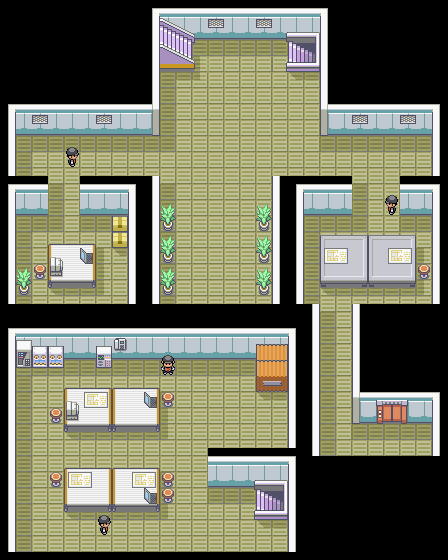
\includegraphics[width=\linewidth]{Kanto_Rocket_Hideout_F1_Map_24bpp.png}
\captionof{figure}{Team Rocket Hideout as depicted in Pokémon FireRed.}
\label{Fig:Style1A}

\end{figure} 

\end{document}
